\section*{Appendix A}
\addcontentsline{toc}{section}{\numberline{}Appendix A}

\subsection{Introduction}

Atmos2 is a library that adds synchronization to models in JavaScript applications. 

Its goal is to make user interfaces very responsive by hiding the networking. 

\subsubsection{Overview}

\begin{figure}[htbp]
  \centering
    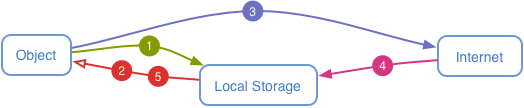
\includegraphics[width=4in]{figures/atmos-02.png}
  \caption{Overview of Atmosphere functioning}
  \label{fig:figures_atmos-02}
\end{figure}

\begin{enumerate}
\item Object is saved to local storage. 
\item User interface is immediately updated
\item Request is made to update the object on the remote side
\item Local version is updated from the response
\item User interface is updated according to changes received from the server
\end{enumerate}



\subsubsection{API Example}

**Fetching objects from remote source**

    MyModel.sync(remote: true)

Fetches remote data and persists them in a local collection. Triggers an event on the model, so that the user interface could be updated.

**Saving object**

    myRecord.save(remote: true)
    
Stores changes in local storage and makes remote request. When the request is done, updates the local data and triggers event to update the user interface.

\subsubsection{Features}

- **API configuration**: Advanced options of configuring API. So far used with typical Rails app and Google Tasks API.
- **Fetching and caching**: Objects can be fetched and cached in local storage.
- **Sync and posting**: When object is changed, it is saved locally, then posted to the server.
- **Offline usage**: The design allows for building offline applications.
- **Live updating**: Comes with [atmos2-server](https://github.com/vojto/atmos2-server) which is lightweight Node.js proxy for updating objects in real time. 

\subsubsection{Notes}

The current implementation uses the model layer of [Spine.js](http://spinejs.com/). All the code that works with Spine is encapsulated in the [AppContext class](https://github.com/vojto/atmos2/blob/master/src/app_context.coffee), which is 80 lines of CoffeeScript.

\subsection{Getting Started}

Take existing Spine app or create a new one.

**Install atmos2**

`git clone git://github.com/vojto/atmos2.git node_modules/atmos2`

**Update slug.json**

Add these modules to your `slug.json`:

    "dependencies": [
		…
    	"atmos2",
    	"atmos2/lib/spine"
  	],

**Setup the model**

Let's say this is your current Spine model:

    class Task extends Spine.Model
      @configure 'Task', 'title', 'kind', 'selfLink'

**Extend the model**

All you have to do is require Atmosphere's Spine adapter, and extend model with it.

    require('atmos2/lib/spine')
    
    class Task extends Spine.Model
      @configure 'Task', 'title', 'kind', 'selfLink'
      @extend Spine.Model.Atmosphere

Atmosphere will automatically use the local storage.

**Set up the synchronizer**

Do this somewhere, where it will be executed before anything else.

    Atmos = require('atmos2')
    
    atmos = new Atmos
    atmos.resourceClient.base = "https://www.googleapis.com/tasks/v1/users/@me"

As you can see, this example will work with Google Tasks API. But first, Atmosphere needs more information.

    atmos.resourceClient.routes =
      Task:
        index: "/lists"
    atmos.resourceClient.addHeader "Authorization", "OAuth #{token}"
    atmos.resourceClient.IDField = "id"
    atmos.resourceClient.dataCoding = "json"
    atmos.resourceClient.itemsFromResult = (result) -> result.items
    
* `routes` specifies path that will be hit on actions: index, create, update, delete. (TODO: Add others to the example.)
* `addHeader` adds header to every request. In this case, we're adding OAuth Authorization, which we've taken care of someplace else, so we have a token.
* `IDField` every retrieved object must have an ID. Some APIs expose this ID in field `id`, others `identifier`, so this settings lets you set it. If a record with empty ID will be retrieved, Atmosphere will throw an error.
* `dataCoding` can be `form` or `json`, specifies in what format will be outgoing data encoding and sent. (Also, what `Content-Type` will be used)
* `itemsFromResult` is a function that will be used to get the items from object decoded from response JSON. In this case, we receive a JSON that looks like this: `{items: [...]}`, so we need to tell Atmosphere how to look for actual records.


\subsubsection{Fetching objects}

    Task.sync(remote: true)

This will first fetch data from local storage triggering the `refresh` event, then make the network request, update local data, and trigger `refresh` event again.

\subsubsection{Sending objects}

    task = new Task({title: "Task 2"})
    task.save(remote: true)

Calling `save` will first save the object locally, then it will make network request to save it again. `create` action will be used.

If you call `save` on already saved object, `update` action will be used. Atmosphere keeps track of all objects you saved with `remote` flag to differentiate between objects that have been sent previously and those once that haven't.